\chapter{Introdu\c{c}\~ao}
\label{cap:introducao}

A experimenta\c{c}\~ao \`a campo ocupa papel fundamental nos programas de melhoramento vegetal, pois permite avaliar materiais gen\'eticos sob condi\c{c}\~oes reais de cultivo. Esse processo depende da observa\c{c}\~ao sistem\'atica de caracter\'isticas fenot\'ipicas relacionadas ao desenvolvimento, \`a produtividade e \`a adapta\c{c}\~ao das plantas. \`A medida que aumenta o n\'umero de gen\'otipos, \'areas e momentos de avalia\c{c}\~ao, cresce tamb\'em a demanda por m\'etodos capazes de ampliar a aquisi\c{c}\~ao e o processamento das informa\c{c}\~oes experimentais. Esse cen\'ario tem impulsionado estrat\'egias de fenotipagem de alto rendimento, nas quais sensores e m\'etodos computacionais s\~ao empregados para reduzir a depend\^encia de avalia\c{c}\~oes exclusivamente manuais \citep{araus2014}.

As imagens de sensoriamento remoto constituem uma das fontes utilizadas nesse processo. A literatura agr\'icola contempla tanto aquisi\c{c}\~oes orbitais quanto imagens obtidas por plataformas a\'ereas de baixa altitude. Em experimentos com forrageiras tropicais, estudos realizados em colabora\c{c}\~ao com a \textbf{Embrapa Gado de Corte} (Centro Nacional de Pesquisa de Gado de Corte) e a \textbf{UFMS - Universidade Federal de Mato Grosso do Sul} investigam imagens obtidas por VANT (Ve\'iculo A\'ereo N\~ao Tripulado) para estimativa de biomassa e rendimento de mat\'eria seca \citep{castro2020,oliveira2021}. Esses trabalhos caracterizam o dom\'inio de aplica\c{c}\~ao, e os dados desta qualifica\c{c}\~ao re\'unem imagens orbitais e ortomosaicos (mapa de alta resolu\c{c}\~ao formado pela uni\~ao de v\'arias fotografias a\'ereas) obtidos por drones.

No ensaio agron\^omico, entretanto, n\~ao basta reconhecer vegeta\c{c}\~ao na imagem. Os materiais avaliados s\~ao distribu\'idos em parcelas que ocupam posi\c{c}\~oes previamente definidas no delineamento experimental. Para que uma informa\c{c}\~ao extra\'ida da imagem possa ser relacionada ao gen\'otipo, tratamento ou unidade correspondente, \'e necess\'ario localizar e delimitar cada parcela e estabelecer sua rela\c{c}\~ao com o croqui, que representa a disposi\c{c}\~ao planejada das unidades experimentais. A identifica\c{c}\~ao das parcelas constitui, portanto, uma etapa anterior \`a extra\c{c}\~ao e \`a compara\c{c}\~ao de caracter\'isticas fenot\'ipicas.

Parte desse trabalho pode ser realizada manualmente ou com o apoio de ferramentas voltadas \`a manipula\c{c}\~ao de imagens georreferenciadas. O \textbf{FIELDimageR}, por exemplo, disponibiliza recursos para gera\c{c}\~ao e ajuste de grades sobre ortomosaicos destinados \`a an\'alise de experimentos agr\'icolas \citep{matias2020}. Ainda assim, opera\c{c}\~oes de posicionamento, dimensionamento e corre\c{c}\~ao das regi\~oes de interesse podem exigir interven\c{c}\~ao humana, principalmente quando diferentes \'areas ou per\'iodos precisam ser processados.

A localiza\c{c}\~ao autom\'atica de parcelas experimentais tem sido investigada por diferentes estrat\'egias, que v\~ao da segmenta\c{c}\~ao semiautomatizada a partir de imagens a\'ereas \citep{robb2020} ao ajuste de uma grade associada ao delineamento \citep{khan2019,mardanisamani2021}, ao acoplamento entre redes convolucionais e processamento geom\'etrico \citep{han2024} e \`a segmenta\c{c}\~ao orientada para parcelas rotacionadas \citep{zhang2025}. Em conjunto, esses trabalhos mostram que a extra\c{c}\~ao de parcelas depende n\~ao apenas da evid\^encia visual, mas tamb\'em da geometria e da disposi\c{c}\~ao espacial das unidades experimentais; a rela\c{c}\~ao entre eles e o procedimento adotado nesta pesquisa \'e retomada na Se\c{c}\~ao~\ref{sec:relacao-literatura}.

Outro aspecto relevante \'e a composi\c{c}\~ao dos dados empregados no treinamento dos modelos. Trabalhos de detec\c{c}\~ao supervisionada que priorizam exemplos dif\'iceis, organizam as amostras por dificuldade ou selecionam subconjuntos representativos indicam que as amostras de treinamento n\~ao precisam ser tratadas como igualmente informativas e que sua sele\c{c}\~ao pode ser investigada como parte do processo de aprendizagem \citep{shrivastava2016,wang2018,lee2024}. Essa literatura \'e detalhada na Se\c{c}\~ao~\ref{sec:generalizacao-dependencia}.

\'E nesse contexto que se insere o trabalho, desenvolvido no \^ambito do projeto \textbf{PhenoSight}, conduzido de forma colaborativa com a Embrapa Gado de Corte, sob orienta\c{c}\~ao do professor Dr. Edson Takashi Matsubara. O objetivo deste projeto \'e criar ferramentas de vis\~ao computacional que possam identificar, delimitar, quantificar, posicionar e arranjar \'areas de cultivo de forrageiras para pesquisa. Para tanto, foram empregadas imagens provenientes de sat\'elites e de drones, com subsequente avalia\c{c}\~ao da conex\~ao entre as informa\c{c}\~oes usadas no aprendizado das ferramentas, a efic\'acia da detec\c{c}\~ao e a organiza\c{c}\~ao geogr\'afica das parcelas.

\begin{figure}[htb]
  \centering
  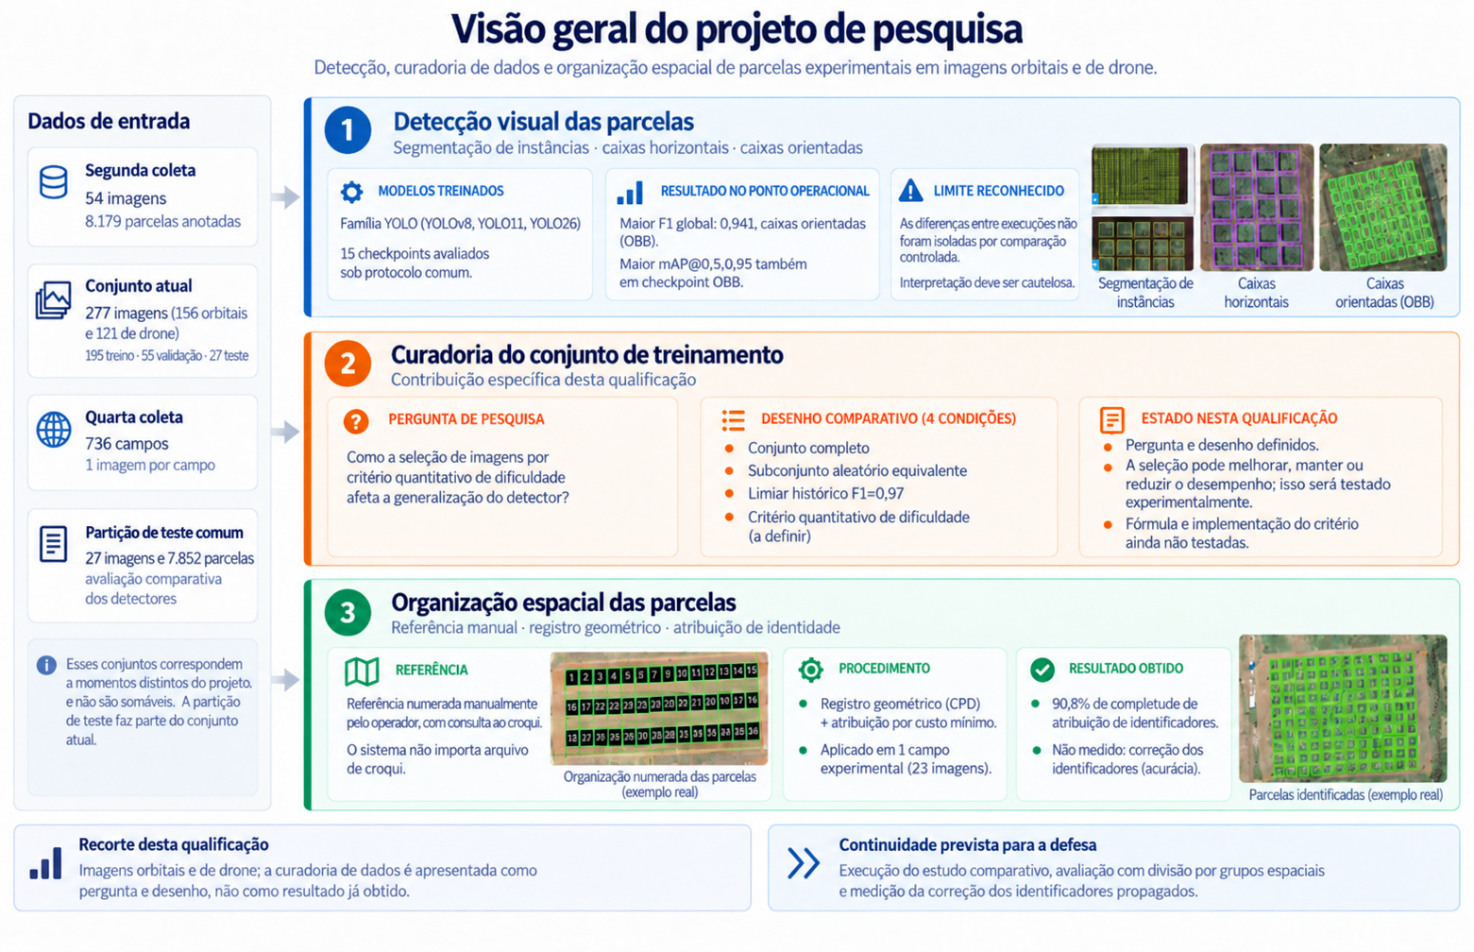
\includegraphics[width=0.95\textwidth]{figuras/figura01.png}
  \caption{Vis\~ao geral das principais frentes metodol\'ogicas do projeto de pesquisa.}
  \label{fig:visao-geral-frentes}
  \fonte{Elaborado pelo autor (2026).}
\end{figure}

O acervo anotado foi ampliado ao longo do projeto. A primeira coleta, foi de 35 imagens e 3.444 parcelas, mas n\~ao catalogada, j\'a a segunda coleta reuniu 54 imagens e 8.179 parcelas anotadas em formato poligonal; o conjunto usado nos experimentos mais recentes t\^em 277 imagens, orbitais e de drone, com 51.245 parcelas divididas entre treinamento, valida\c{c}\~ao e teste; e a coleta em andamento, com imagens orbitais de 1.045 campos experimentais e novos ortomosaicos obtidos por drone, que deve ultrapassar mais de 1.200 imagens de campo. Esses n\'umeros correspondem a momentos distintos do projeto e n\~ao s\~ao som\'aveis. A composi\c{c}\~ao e o uso de cada conjunto s\~ao detalhados na se\c{c}\~ao ``Metodologia''.

Ao longo desse desenvolvimento, foram investigadas diferentes formas de representar e localizar as parcelas, incluindo segmenta\c{c}\~ao de inst\^ancias, detec\c{c}\~ao por caixas delimitadoras horizontais, detec\c{c}\~ao por caixas delimitadoras orientadas e uma abordagem alternativa baseada em mapas de confian\c{c}a. Tamb\'em foi estudado, um classificador auxiliar, relacionado \`a dificuldade das imagens e procedimentos de associa\c{c}\~ao espacial destinados a preservar a identifica\c{c}\~ao das parcelas entre imagens de uma mesma \'area \`a campo. Essas frentes permitiram avan\c{c}ar na identifica\c{c}\~ao e na organiza\c{c}\~ao das parcelas visualmente detect\'aveis, embora situa\c{c}\~oes em que a estrutura experimental prev\^e uma posi\c{c}\~ao sem detec\c{c}\~ao correspondente ainda exijam tratamento espec\'ifico.

\begin{figure}[htb]
  \centering
  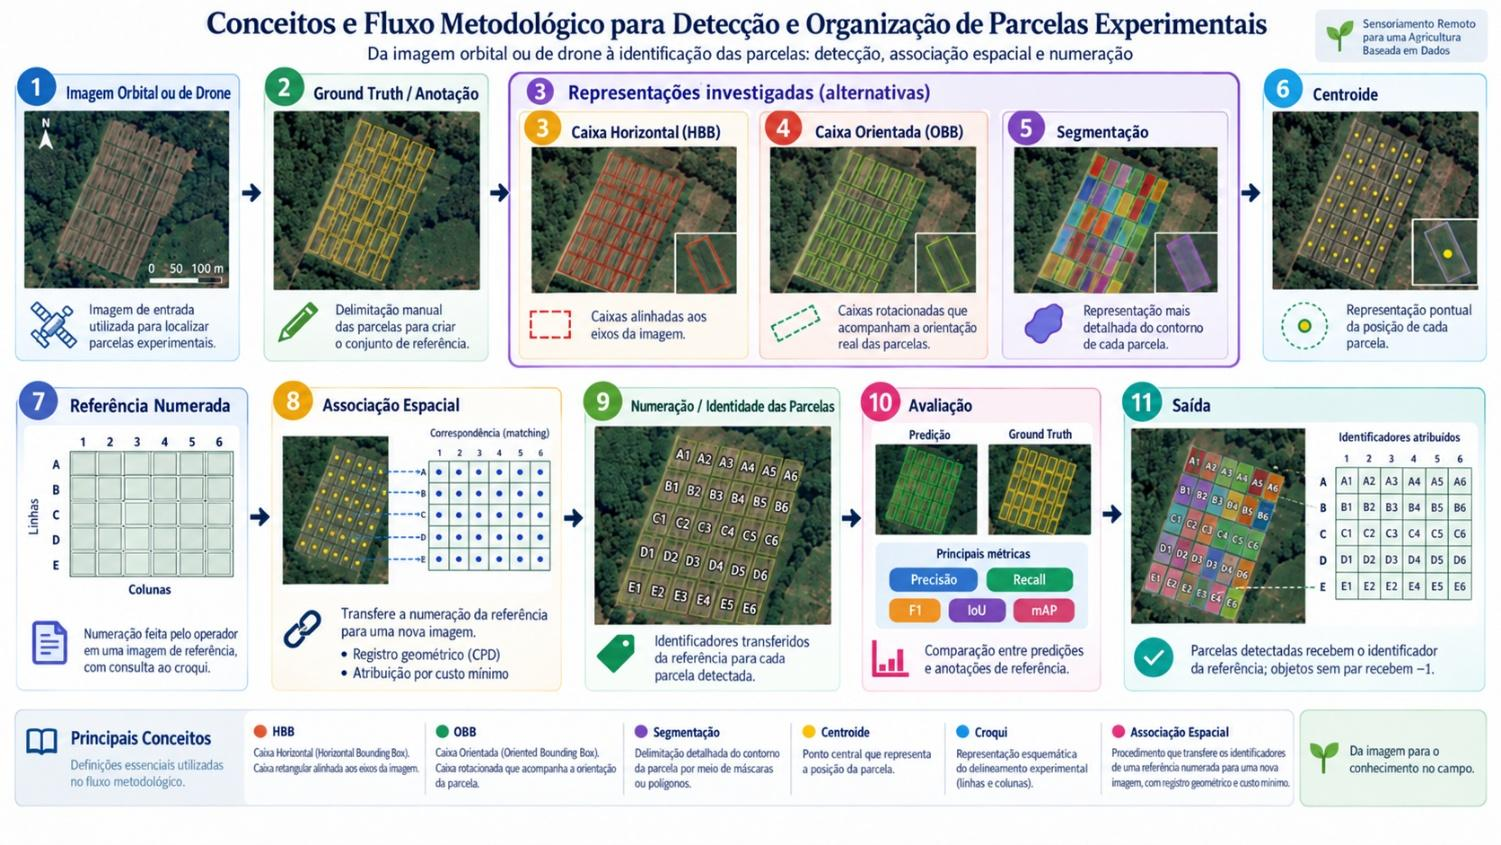
\includegraphics[width=0.95\textwidth]{figuras/figura02.jpg}
  \caption{Conceitos e fluxo metodol\'ogico para detec\c{c}\~ao e organiza\c{c}\~ao de parcelas experimentais em imagens orbitais e de drone.}
  \label{fig:conceitos-fluxo}
  \fonte{Elaborado pelo autor (2026).}
\end{figure}

A evolu\c{c}\~ao dos experimentos revelou tamb\'em uma quest\~ao metodol\'ogica relacionada \`a pr\'opria composi\c{c}\~ao do conjunto de treinamento. Essa composi\c{c}\~ao n\~ao foi originalmente tratada como uma vari\'avel experimental controlada. Em 2025, as imagens receberam manualmente n\'iveis de dificuldade, e as de n\'ivel mais alto foram replicadas no treinamento de parte dos modelos, sem compara\c{c}\~ao com um treinamento n\~ao ponderado nas mesmas condi\c{c}\~oes. Posteriormente, um limite hist\'orico da m\'etrica F1-Score igual a 0,97, por indica\c{c}\~ao do professor, foi empregado para classificar as imagens de acordo com a complexidade exibida ao detector, com o prop\'osito de criar os r\'otulos para um classificador secund\'ario; tal m\'etodo n\~ao foi planejado nem examinado como t\'atica para escolher as imagens usadas no treino do detector. Da mesma forma, foram encontradas imagens da mesma regi\~ao em divis\~oes distintas do conjunto de dados, o que sublinha a import\^ancia de verificar a generaliza\c{c}\~ao em grupos que n\~ao estiveram envolvidos no treino.

Um ponto importante levantado nesta pesquisa, \'e de como a sele\c{c}\~ao das imagens de treinamento por um crit\'erio quantitativo de instabilidade das predi\c{c}\~oes, estimado fora da amostra, afeta na generaliza\c{c}\~ao do detector de parcelas, em compara\c{c}\~ao com o conjunto completo, com subconjuntos aleat\'orios de mesmo tamanho e com o limiar hist\'orico j\'a mencionado. Com isso, surge a hip\'otese de pesquisa deste trabalho, com um conjunto de dados selecionado atrav\'es deste m\'etodo resultando em um detector com melhor capacidade de generaliza\c{c}\~ao em compara\c{c}\~ao com aqueles criados a partir de conjuntos de dados aleat\'orios de tamanho similar. A an\'alise com o conjunto de dados integral serve para mensurar o impacto da diminui\c{c}\~ao do volume de imagens, sem, no entanto, garantir a preserva\c{c}\~ao do desempenho; a escolha poder\'a tanto aprimorar, manter quanto prejudicar o desempenho, e isso ser\'a verificado atrav\'es de experimentos.

Dito isso, podemos descrever como objetivo geral deste projeto:

Investigar e avaliar m\'etodos de vis\~ao computacional para identificar, localizar e organizar parcelas experimentais de forrageiras em imagens orbitais e de drone, com \^enfase na an\'alise do efeito da composi\c{c}\~ao do conjunto de treinamento sobre a generaliza\c{c}\~ao do detector. Para isso, a trajet\'oria j\'a desenvolvida de detec\c{c}\~ao, segmenta\c{c}\~ao e representa\c{c}\~ao espacial ser\'a articulada a um estudo comparativo controlado de diferentes estrat\'egias de composi\c{c}\~ao dos dados.

Ser\~ao comparados o conjunto completo de imagens, subconjuntos aleat\'orios de mesmo tamanho, como j\'a mencionado, com um limiar hist\'orico, e um crit\'erio de instabilidade das predi\c{c}\~oes adaptado do Variance-based Prediction Score \citep{yagi2025}, por ser similar, sendo um aprendizado supervisionado.

A relev\^ancia dessa investiga\c{c}\~ao, est\'a em tratar a composi\c{c}\~ao do conjunto de treinamento como parte expl\'icita do problema de detec\c{c}\~ao, em vez de restringir a an\'alise \`a escolha da arquitetura ou ao valor final de uma m\'etrica. No contexto aplicado, busca-se produzir evid\^encias sobre como diferentes estrat\'egias de sele\c{c}\~ao das imagens afetam o desempenho em dados n\~ao utilizados no ajuste do modelo. Cientificamente, esta pesquisa aproxima a discuss\~ao sobre informatividade e sele\c{c}\~ao de amostras do problema de detec\c{c}\~ao de parcelas agr\'icolas densamente distribu\'idas, sem assumir antecipadamente que exemplos considerados dif\'iceis devam ser exclu\'idos ou priorizados.
